In order to compare the fairness across locks and different sizes we decided to
create a scale from $0$ to $1$ where $0$ is a perfectly fair lock and $1$ is a
lock where only one thread has repeatedly acquired the lock.
To avoid creating a biased measure, we reuse the concept of standard deviation
from statistics, that we re-scale for our purposes.
In particular, we call our measure $U$ for \textit{Unfairness}:
$$
  U = \frac{\sqrt{n}}{\sum_{i = 1}^{n} k_i} \operatorname{sd}(k_i)
    = \frac{\sqrt{n}}{\sqrt{n-1}} \frac{\sqrt{\sum_{i = 1}^{n} (k_i - \bar{k})^2}}{\sum_{i = 1}^{n} k_i}
$$
where $n$ is the number of threads and $k_i$ is the number of locks acquired by thread $i$.

Using this definition we inherit the following properties from the standard deviation:
\begin{itemize}
  \item When all threads acquire the same amount of locks then
    $k_i = \bar{k} \forall i$, then $\operatorname{sd}(k_i) = 0 $ and the result
    is zero.
  \item When counting elements, the standard deviation is maximal when only one
    element is maximal.
    We can show that the maximum of $U$ is 1, by setting $k_i = 0 \forall i \neq j$ and $k_j \neq 0$:
    \begin{align*}
      U &= \frac{\sqrt{n}}{\sqrt{n-1}} \frac{\sqrt{(n-1)(\bar{k})^2 + (k_j - \bar{k})^2}}{k_j} \\
        &= \frac{\sqrt{n}}{\sqrt{n-1}} \frac{\sqrt{(n-1)(k_j/n)^2 + (k_j - k_j/n)^2}}{k_j} \\
        &= \frac{1}{k_j} \sqrt{\frac{n}{n-1} \left[(n-1)\frac{k_j^2}{n^2} + \frac{k_j^2}{n^2}(n - 1)^2 \right]} \\
        &= \frac{1}{k_j} \sqrt{n \left[\frac{k_j^2}{n^2} + \frac{k_j^2}{n^2}(n - 1) \right]} \\
        &= \frac{1}{k_j} \sqrt{n^2\frac{k_j^2}{n^2}} = 1.
    \end{align*}
\end{itemize}

This measure allows to meaningfully compare the (un)fairness across
various implementations and with different sizes in figure \ref{fig:fairness-all}.

We notice immediately that the TAS, TTAS, and OpenMP locks are highly unfair.
In the collected data most of the executions are characterised by one or two
threads mostly getting the lock.
We can then exclude them from the plot to distinguish and better visualize the custom locks in figure \ref{fig:fairness-no-tas}. Note that now the y-axis value are very close to zero.

Between these, we have that the Bakery and derivatives behave very similarly, with
an extremely low unfairness, while the Peterson Tree and Filter lock present some peaks.
In particular we can observe a positive correlation between unfairness and size of
the cluster for the Peterson lock.

This is in line with the theory, in fact the TAS and TTAS locks are extremely
opportunistic and all threads wait in the same queue, no matter if they have
just exited the CS or have been trying to access for a long while.
The Filter and Peterson Tree Lock do not provide fairness guarantees, but still
implement a queue, that prevent such behaviour from happening, and this is
reflected in a slightly uneven thread acquisition distribution.
Bakery, Lamport, and Boulangerie are instead FIFO, and this is reflected in
their extremely fair behaviour. The fluctuation that is seen at the lower end
of the graph is due to integer division: by doing only 1024 iterations some
set of threads will get one iteration more if 1024 is not divisible by $n$, the 
number of threads.

\begin{figure}[H]
  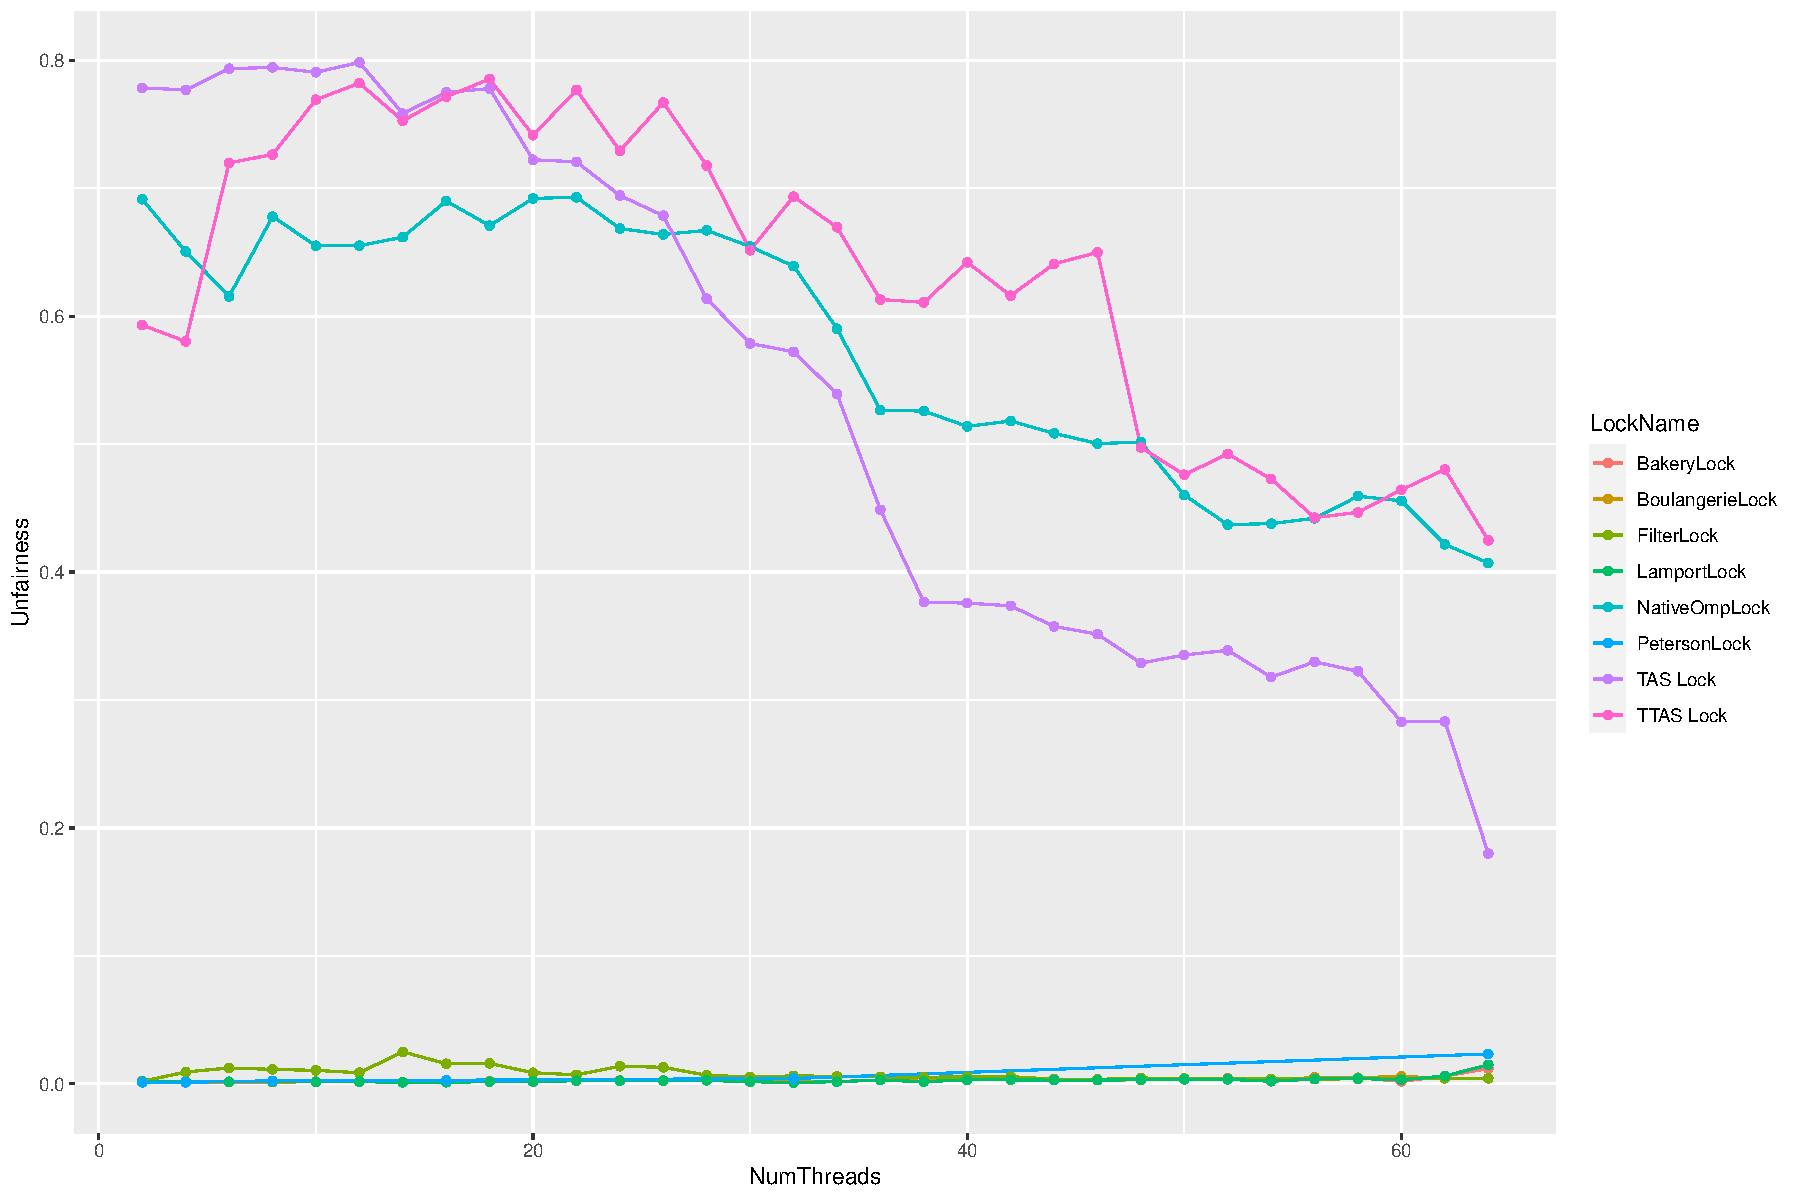
\includegraphics[width=\textwidth]{fig/fairness_all}
  \caption{Fairness for all implemented locks}
  \label{fig:fairness-all}
\end{figure}

\begin{figure}[H]
  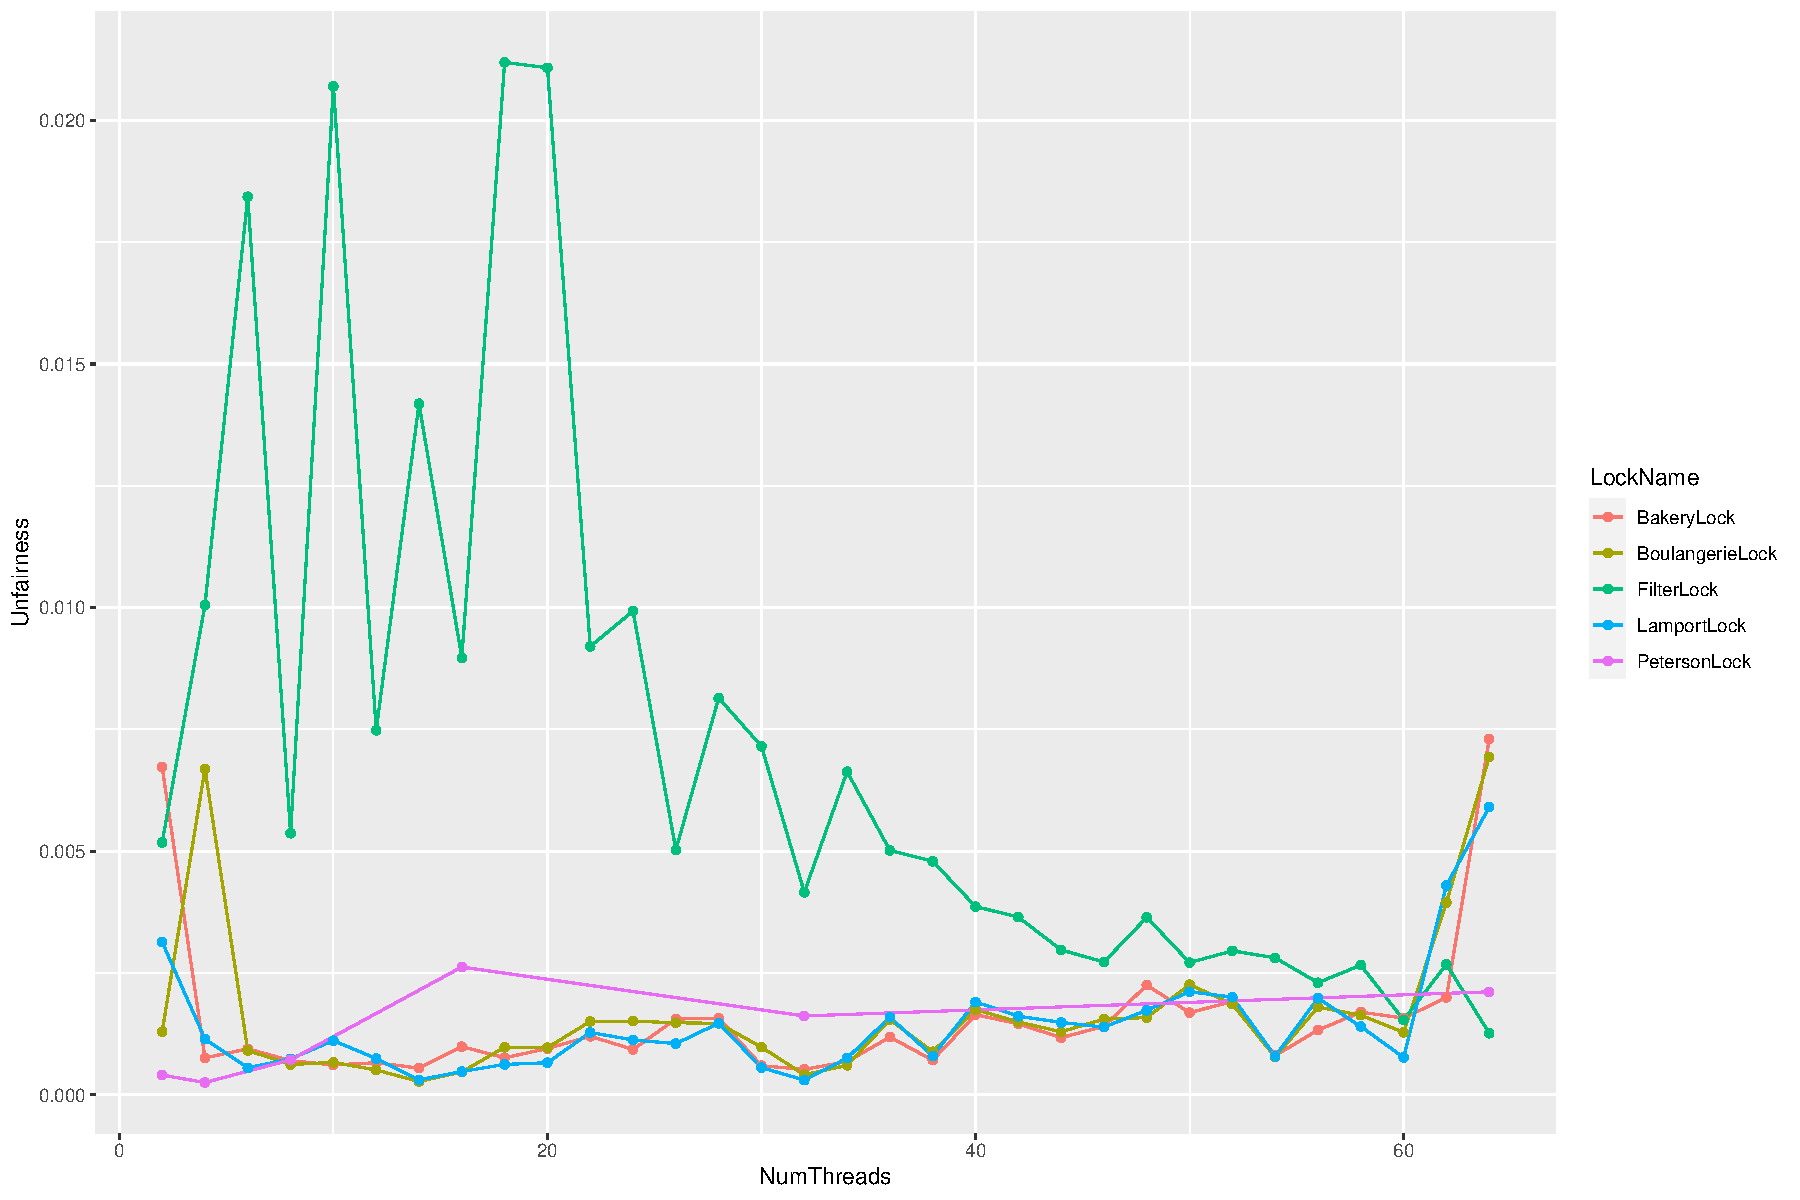
\includegraphics[width=\textwidth]{fig/fairness_no_tas}
  \caption{Fairness for custom locks}
  \label{fig:fairness-no-tas}
\end{figure}
